%%%%%%%%%%%%%%%%%%%%%%%%%%%%%%%%%%%%%%%%%%%%%%%%%%%%%%%%%%%%%%%%%%%%%%%%%%%%%%%

\documentclass[12pt,twocolumn,tighten]{aastex62}
%\documentclass[12pt,twocolumn,tighten,trackchanges]{aastex62}
\usepackage{amsmath,amstext,amssymb}
\usepackage[T1]{fontenc}
\usepackage{apjfonts}
\usepackage[figure,figure*]{hypcap}
\usepackage{graphics,graphicx}
\usepackage{hyperref}
\usepackage{natbib}

\renewcommand*{\sectionautorefname}{Section} %for \autoref
\renewcommand*{\subsectionautorefname}{Section} %for \autoref

%% Reintroduced the \received and \accepted commands from AASTeX v5.2.
%% Add "Submitted to " argument.
\received{\today}
\revised{---}
\accepted{---}
\submitjournal{AAS journals.}
\shorttitle{Against PTFO$\,$8-8695b}

\begin{document}

\defcitealias{bouma_wasp4b_2019}{B19}

\title{Against the Planetary Interpretation of PTFO$\,$8-8695b}

\correspondingauthor{L. G. Bouma}
\email{luke@astro.princeton.edu}

%
% key authors:
%
\author[0000-0002-0514-5538]{L. G. Bouma}
\affiliation{ Department of Astrophysical Sciences, Princeton
University, 4 Ivy Lane, Princeton, NJ 08540, USA}
%
\author[0000-0002-4265-047X]{J. N. Winn}
\affiliation{ Department of Astrophysical Sciences, Princeton
University, 4 Ivy Lane, Princeton, NJ 08540, USA}

%
% contributing authors: alphabetical
%
% \author[0000-0001-8638-0320]{A. W. Howard}
% \affiliation{Cahill Center for Astrophysics, California Institute of
% Technology, Pasadena, CA 91125, USA}
% %
% \author[0000-0002-2532-2853]{S. B. Howell}
% \affiliation{NASA Ames Research Center, Moffett Field, CA 94035, USA}
% %
% \author[0000-0002-0531-1073]{H. Isaacson}
% \affiliation{Astronomy Department, University of California, Berkeley,
% CA 94720, USA}
% %
% \author{H. Knutson}
% \affiliation{Division of Geological and Planetary Sciences, California
% Institute of Technology, Pasadena, CA 91125, USA}
% %
% \author[0000-0001-7233-7508]{R. A. Matson}
% \affiliation{U.S. Naval Observatory, Washington, DC 20392, USA}
% %

\begin{abstract}
  PTFO$\,$8-8695b could be the youngest, shortest-period 
  hot Jupiter known.  However it has not been shown to be a planet.
  TESS recently observed PTFO$\,$8-8695 for one month.
  The TESS lightcurve shows that the dominant variability in this
  system is a sinusoidal modulation with a ``long'' period $P_{\rm
  \ell}$
  of 11.96 hours, likely caused by stellar rotation.
  Also present is a complex signal, previously identified as the
  planet candidate, that repeats with a ``short'' period $P_{\rm s}$ of
  10.74 hours.
  The ``long'' and ``short'' signals show the expected beat every 4.48
  days.
  There is a dip in the complex, short-period signal.
  However ground-based photometry from the past decade shows that the
  orbital phase of the dip seems to have instantaneously jumped, at
  least once, and maybe twice.
  The TESS epoch of the dip is consistent with recent observations by
  Tanimoto et al., and differs from the discovery epoch by 5.14 hours.
  Planets do not ``jump'' in orbital phase.
  Given the available evidence,
  PTFO$\,$8-8695 seems consistent with the
  ``transient dipping'' phenomenology observed in many young M dwarfs.
  It seems rather unlikely to be a planet.
\end{abstract}

%TODO
\keywords{}

%%%%%%%%%%%%%%%%%%%%%%%%%%%%%%%%%%%%%%%%%%%%%%%%%%%%%%%%%%%%%%%%%%%%%%%%%%%%%%%

\section{Introduction}
If PTFO$\,$8-8695b were a planet, it would be exceptional.
A transiting hot Jupiter, orbiting a $\approx$3$\,$Myr old M dwarf
in ORION would make it the youngest hot Jupiter known.
Its orbital period of only 12 HOURS would also make it the shortest
period hot Jupiter known.

% Section~\ref{sec:observations} of this paper presents all of the
% available transit data as well as the new radial velocity and speckle
% imaging observations.  Section~\ref{sec:analysis} describes our
% analysis of the data, and our interpretation that WASP-4 is being
% pulled around by a brown dwarf or low-mass star.
% Section~\ref{sec:discussion} places this result within the context of
% orbital decay searches, and points out that line-of-sight
% accelerations will be a relatively common type of ``false positive.''
% Section~\ref{sec:conclusions} offers concluding remarks.

\section{The Data}
\label{sec:observations}

\subsection{Observations}

PTFO 8-8695 was observed by TESS with Camera 1, CCD 1, from December
15, 2018 to January 6, 2019, during the sixth sector of science
operations.  The star is designated TIC 264461976 in the TESS Input
Catalog \citep{stassun_TIC_2018,stassun_TIC8_2019}.  The pixel data
for an $11\times11$ array surrounding PTFO 8-8695 were averaged into
2-minute stacks by the onboard computer.  Each 2048$\times$2048 image
from the CCD was also averaged into 30-minute stacks, and saved as a
``full frame image'' (FFI).

The 2-minute stacks for PTFO 8-8695 were then reduced to lightcurves
by the Science Processing Operations Center (SPOC) at NASA
Ames~\citep{jenkins_tess_2016}.  Our main analysis used the resulting
Presearch Data Conditioning (PDC) lightcurve.  The PDC lightcurve
aperture used pixels chosen to maximize the SNR of the total flux of
the target \citep{smith_kepler_apertures_2017}.  Non-astrophysical
variability was removed through the methods discussed by
\citet{smith_kepler_PDC_2017}.

As an independent check on the shorter cadence SPOC light-curve, we
separately processed the 30-minute image stacks as part of the Cluster
Difference Imaging Photometric Survey (CDIPS;
\citep{bouma_cluster_2019}).  The CDIPS lightcurve used a circular
aperture with radius 1 pixel.

For data cleaning, we removed all points with non-zero quality flags
\citep[{\it e.g.},][]{tess_data_product_description_2018}.  We also
masked out the first and last 6 hours of each orbit, since there is
often systematic red noise during those times.  Both the CDIPS and PDC
lightcurves showed a clear discontinuous ``jump'' in the last few days
of orbit 20, which seemed likely to be an instrumental systematic.  We
correspondingly masked out times from BJD 2458488.3 until the end of
the orbit.  The PDC lightcurve initially had 15{,}678 points.  The
quality cut removed 854, masking the orbit edges removed 716, and
removing the final few days of orbit 20 removed 1079.  83\% of the
highest-quality data remained.

We normalized these points by dividing out the median flux. We then
subtracted by unity to simplify subsequent analysis.  Many of these
and subsequent processing steps were performed using
\texttt{astrobase}~\citep{bhatti_astrobase_2018}. 


\subsection{Visual Inspection}

Our initial inspection of the lightcurve, in both its 2-minute PDCSAP
and 30-minute FFI forms, revealed an obvious beat signal
(Figure~\ref{fig:splitsignal}, top panel).

As a precursor to more detailed analysis, we calculated generalized
Lomb-Scargle periodograms using \texttt{astrobase}
\citep{lomb_1976,scargle_studies_1982,vanderplas_periodograms_2015,bhatti_astrobase_2018}.
The two largest peaks in the Lomb-Scargle periodogram of the
lightcurve were clearly separated at $P_{\rm s} \approx 0.448\,{\rm
days}$ and $P_{\rm \ell} \approx 0.499\,{\rm days}$.  The $P_{\rm
\ell}$ peak had the greater power of the two.  Smaller harmonics from
each of these dominant two signals were also present.

% 0.14 = A1+A2
% 0.06 = A1-A2
% 2A1 = 0.20
% -> A1 = 0.1
% 2A2 = 0.08
% -> A2 = 0.04

The beat peak-to-peak amplitude at maximum, when the two signals
constructively interfere, is about 14\%.  At minimum, the peak-to-peak
amplitude is about 6\%.  Assuming the signals are just two sinusoids,
algebra tells us that the peak-to-peak amplitudes should therefore be
10\% for the long-period signal, and 4\% for the short-period signal.
These order-of-magnitude numbers will turn out to be roughly correct.

Initial signal-processing experiments fitting out splines or sinusoids
showed that after subtracting out the long-period signal, the
short-period signal dominated the periodogram, and vice-versa.
However it quickly became clear that it would be beneficial to
simultaneously model the signals separately, in order to preserve the
power at each frequency.




% \subsection{Star and planet parameters}
% \label{sec:system_parameters}
% 
% \begin{deluxetable}{lccc}
% \tabletypesize{\scriptsize}
% \tablecaption{Selected system parameters of WASP-4b\label{tbl:params}}
% \tablenum{1}
% 
% \tablehead{
% \colhead{Parameter} & \colhead{Value} & \colhead{68\% Confidence Interval} & \colhead{Comment}
% }
% 
% \startdata
% {\it Transit/RV parameters:} & & & \\
%   $R_{\rm p}/R_\star$                        & $0.15201$              & $+0.00040$, $-0.00033$      & A \\
%   $i$~[deg]                                  & $89.06$                & $+0.65$, $-0.84$            & A \\
%   $a/R_\star$                                & $5.451$                & $+0.023$, $-0.052$          & A \\
%   $u_{\rm linear}$                           & $0.382$                & ---                         & A \\
%   $u_{\rm quad}$                             & $0.210$                & ---                         & A \\
%   $K$~[m~s$^{-1}$]                           & $241.1$                & $+2.8$, $-3.1$              & B \\
% {\it Stellar parameters:} & & & \\
%   $T_{\rm eff}$~[K]                          & $5400$                 & $\pm 90$                    & C \\
%   $\log g_\star$~[cgs]                       & $4.47$                 & $\pm 0.11$                  & C \\
%   $[{\rm Fe/H}]$                             & $-0.07$                & $\pm 0.19$                  & C \\
%   $F_{\rm bol}$~[erg~cm$^{-2}$~s$^{-1}$]     & $2.802\times10^{-10}$  & $\pm 0.076\times10^{-10}$   & D \\
%   $A_V$~[mag]                                & $0.03$                 & $+0.02, -0.01$              & D \\
%   $\pi$~[mas]                                & $3.7145$               & $0.0517$                    & F \\
%   $R_\star$~[R$_{\odot}$]                    & $0.893$                & $\pm 0.034$                 & E \\
%   $\rho_\star$~[g~cm$^{-3}$]                 & $1.711$                & $+0.022$, $-0.048$          & E \\
%   $M_\star$~[M$_{\odot}$]                    & $0.864$                & $+0.084$, $-0.090$          & E \\
%   $T$ magnitude                              & $11.778$               & $\pm 0.018$                 & G \\
% {\it Planetary parameters:} & & & \\
%   $a$~[AU]                                   & $0.0226$               & $+0.0007$, $-0.0008$        & E \\
%   $M_p$~[M$_{\rm Jup}$]                      & $1.186$                & $+0.090$, $-0.098$          & E \\
%   $R_p$~[R$_{\rm Jup}$]                      & $1.321$                & $\pm 0.039$                 & E \\
% \enddata
% 
% \tablecomments{
%   (A) From phase-folded TESS lightcurve (\S~\ref{sec:measurement}).
%   Orbital periods are in Table~4. The limb darkening parameters were
%   allowed to float around the \citet{claret_limb_2017} prediction, but
%   were unconstrained.
%   (B) \citet{triaud_spin-orbit_2010}.
%   (C) From HARPS spectra \citep{doyle_accurate_2013}.
%   (D) \citet{stassun_accurate_2017}.
%   (E) This work, see \S~\ref{sec:system_parameters}.
%   (F) \citet{gaia_collaboration_gaia_2018}.
%   (G) \citet{stassun_TIC_2018}.
% }
% 
% \vspace{-1cm}
% \end{deluxetable}
% 
% We calculated the stellar and planetary parameters in the following
% way.  We computed the star's spectral energy distribution based on the
% {\it Gaia} DR2 parallax (after making the small correction advocated
% by \citealt{stassun_evidence_2018}) and the broadband magnitudes from
% the available all-sky catalogs: $G$ from {\it Gaia\/} DR2, $B_T$ and
% $V_T$ from {\it Tycho-2}, $BVgri$ from {\it APASS}, $JHK_S$ from {\it
% 2MASS}, and the {\it WISE}~1--4 passbands, thus spanning the
% wavelength range 0.4--22~$\mu$m.
% We adopted the effective temperature
% from the work by \citet{doyle_accurate_2013}, who determined the
% spectroscopic parameters of WASP-4 using high-signal-to-noise
% observations with the High Accuracy Radial-velocity Planet Searcher
% (HARPS).  Then, we determined the stellar radius through the
% combination of the bolometric luminosity and the effective
% temperature, using the Stefan-Boltzmann law.  To determine the stellar
% mass, we first computed the mean stellar density based on the value of
% $a/R_\star$ that gave the best fit to the phase-folded TESS lightcurve
% (for the relevant equation, see \citealt{seager_unique_2003} or
% \citealt{winn_exoplanet_2010}).  The mass was calculated from the
% radius and density, and the orbital distance was also calculated from
% the radius and $a/R_\star$.  The planetary radius was calculated as
% the product of $R_\star$ and $R_{\rm p}/R_\star$.  Finally, the planet
% mass was calculated based on the stellar mass, the radial-velocity
% amplitude observed by \citet{triaud_spin-orbit_2010}, and the orbital
% inclination.
% 
% Table~1 gives the resulting parameters, which we adopted for the
% remaining analysis.  \added{The uncertainties in our derived stellar
% and planetary parameters are propagated according to standard analytic
% formulae, under the assumption that the variables are uncorrelated and
% normally distributed.} Our \added{system} parameters are in agreement
% with those of previous investigators, but have the benefit of
% incorporating the {\it Gaia} parallax
% \citep{wilson_wasp-4b_2008,gillon_discovery_2009,winn_transit_2009,southworth_homogeneous_2011,petrucci_no_2013,huitson_gemini_2017}.
% By comparing the star's luminosity and spectroscopic parameters with
% the outputs of the Yonsei-Yale stellar-evolutionary models, we found
% that WASP-4 is a main-sequence star with an age of approximately
% $7\,{\rm Gyr}$ \added{\citep{demarque_y2_2004}}.



\section{The Model}
\label{sec:analysis}

\begin{figure*}[t]
	\begin{center}
		\leavevmode
		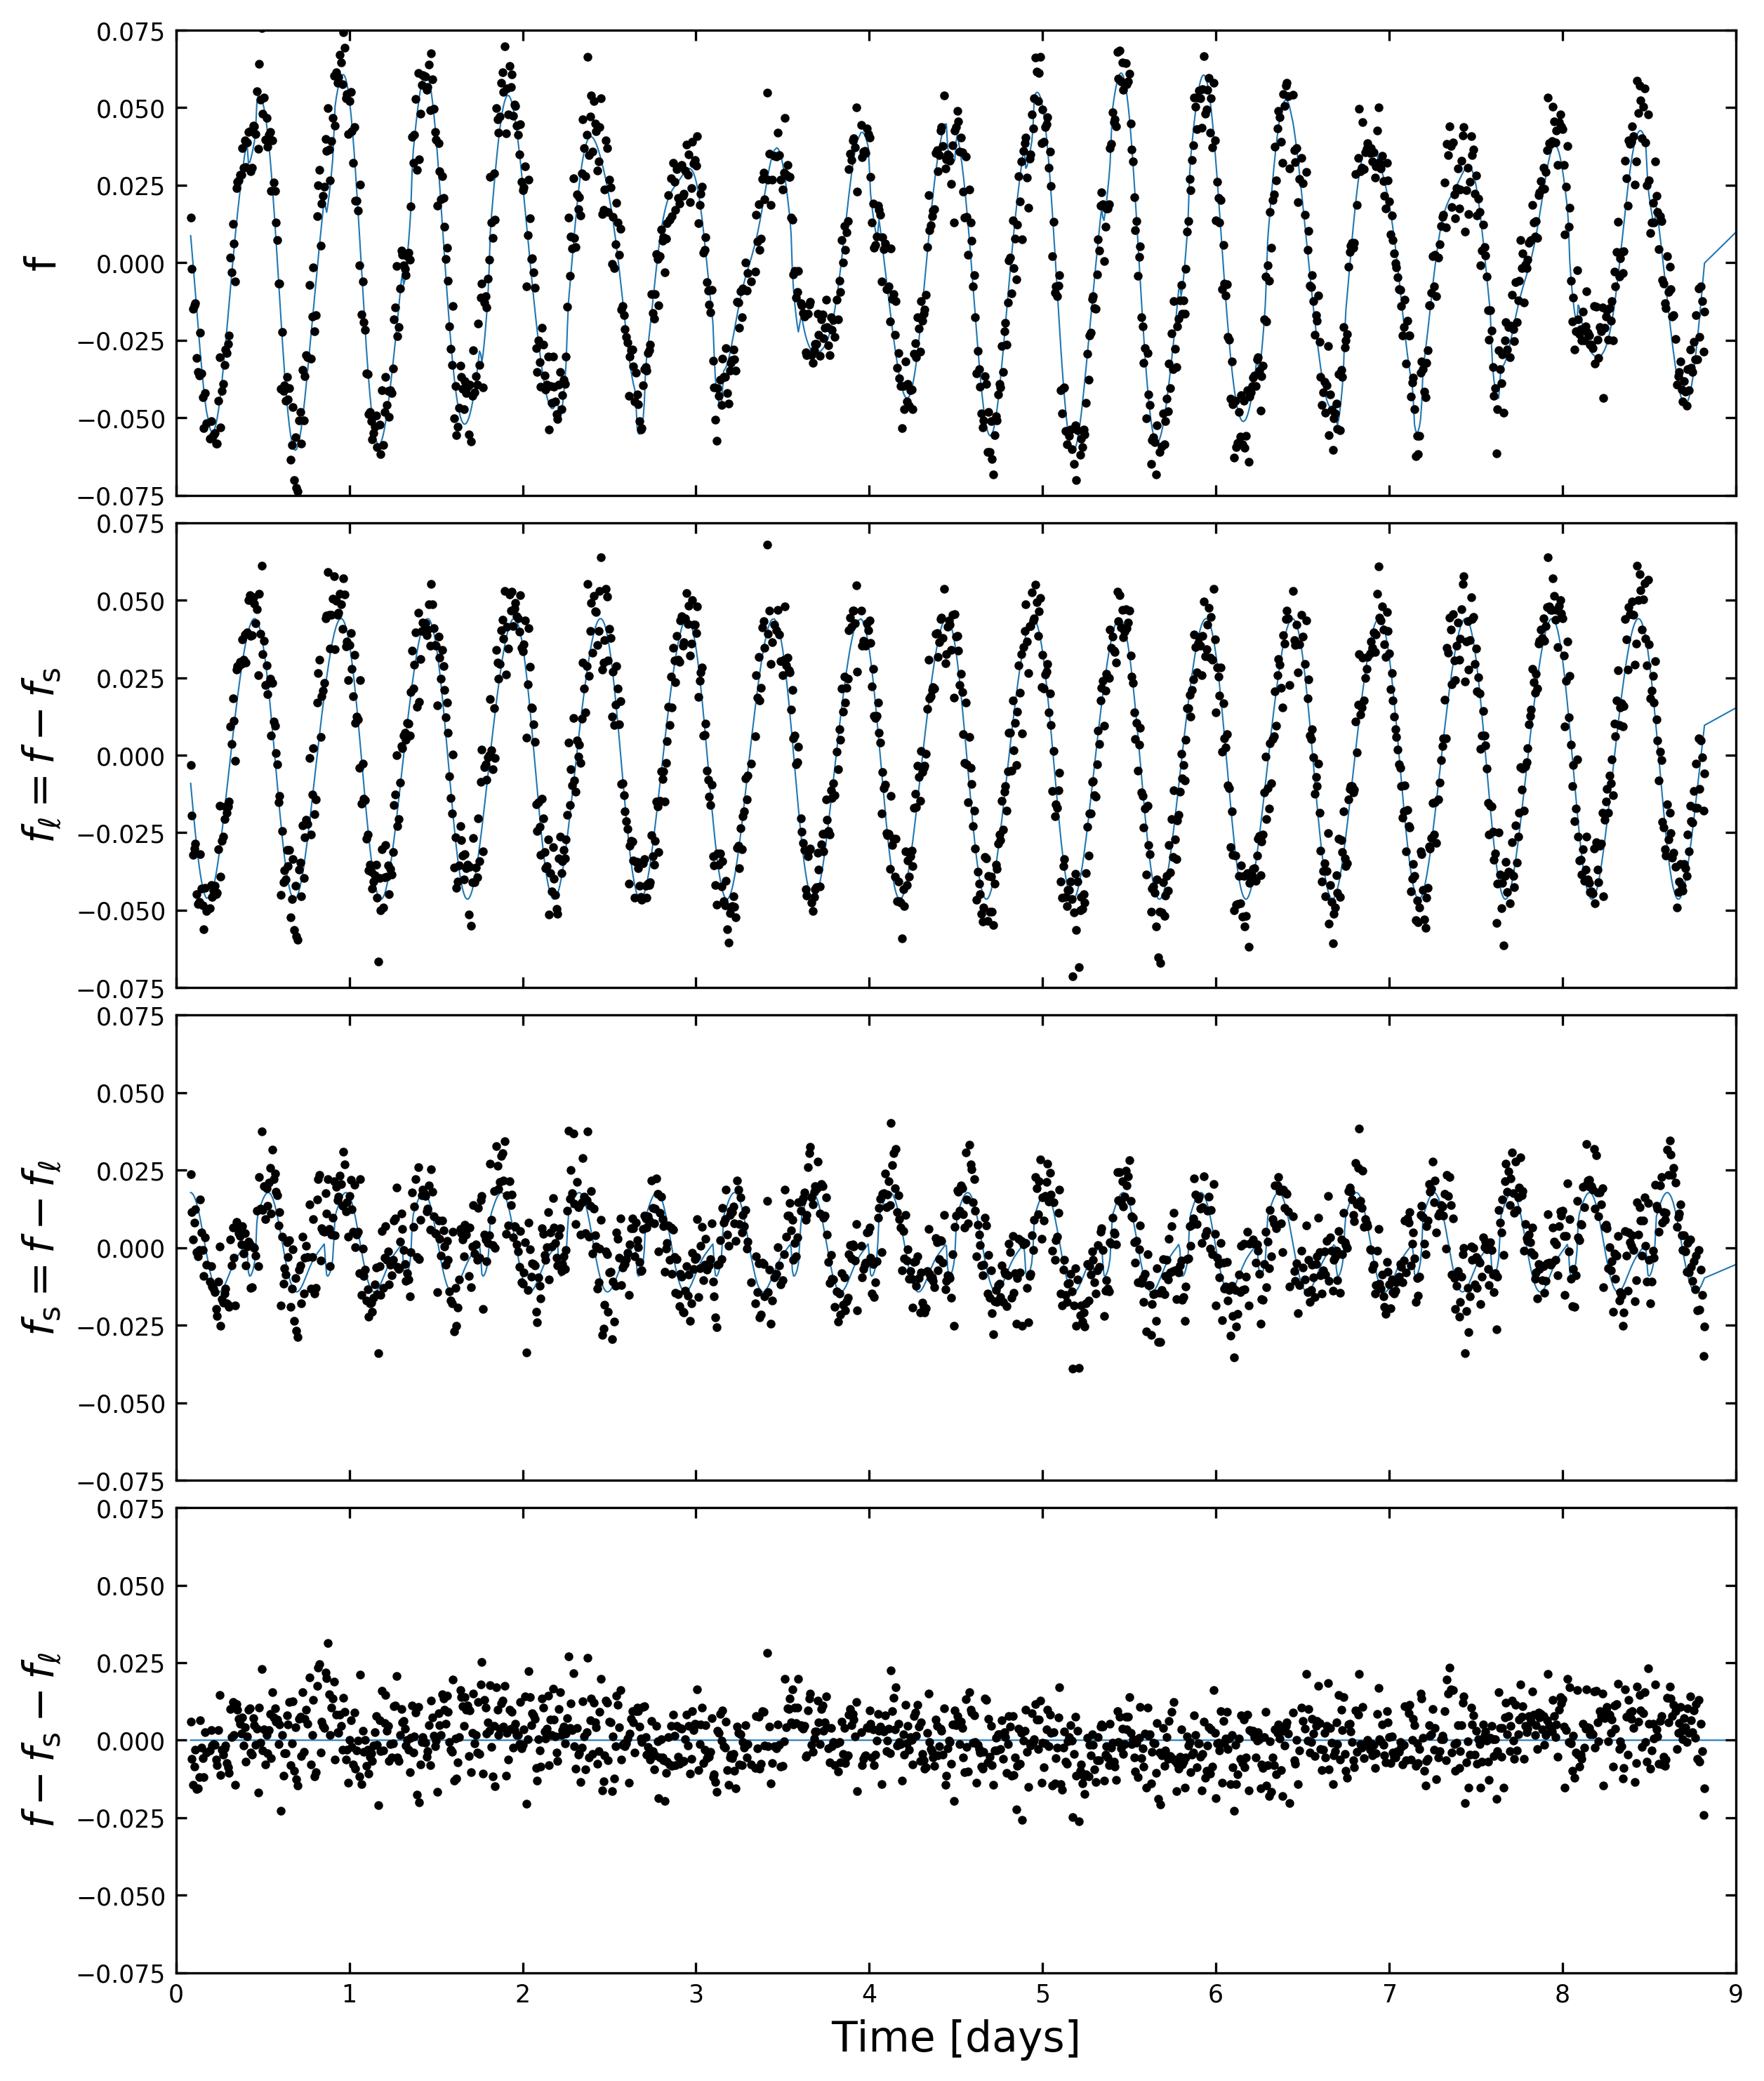
\includegraphics[width=0.98\textwidth]{f1.png}
	\end{center}
	\vspace{-0.7cm}
	\caption{ {\bf TESS lightcurve of PTFO 8-8695 (Sector 6, Orbit 1).}
	{\it Top}: ``Raw'' \texttt{PDCSAP} mean-subtracted relative flux versus time. The beat period of 4.48 days is visible by eye.
	The model plotted underneath the data includes 2 harmonics at the long
	period $P_{\rm \ell}$, plus 2 harmonics and a transit at the short period $P_{\rm s}$.
	{\it Upper middle}: Long-period signal, equal to the raw signal minus the short-period signal.
	{\it Lower middle}: Short-period signal, equal to the raw signal minus the long-period signal.
	{\it Bottom}: residual.
	The data are binned from 2 to 10 minute cadence as a convenience for plotting and fitting.
		\label{fig:splitsignal}
	}
\end{figure*}

\begin{figure*}[t]
	\begin{center}
		\leavevmode
		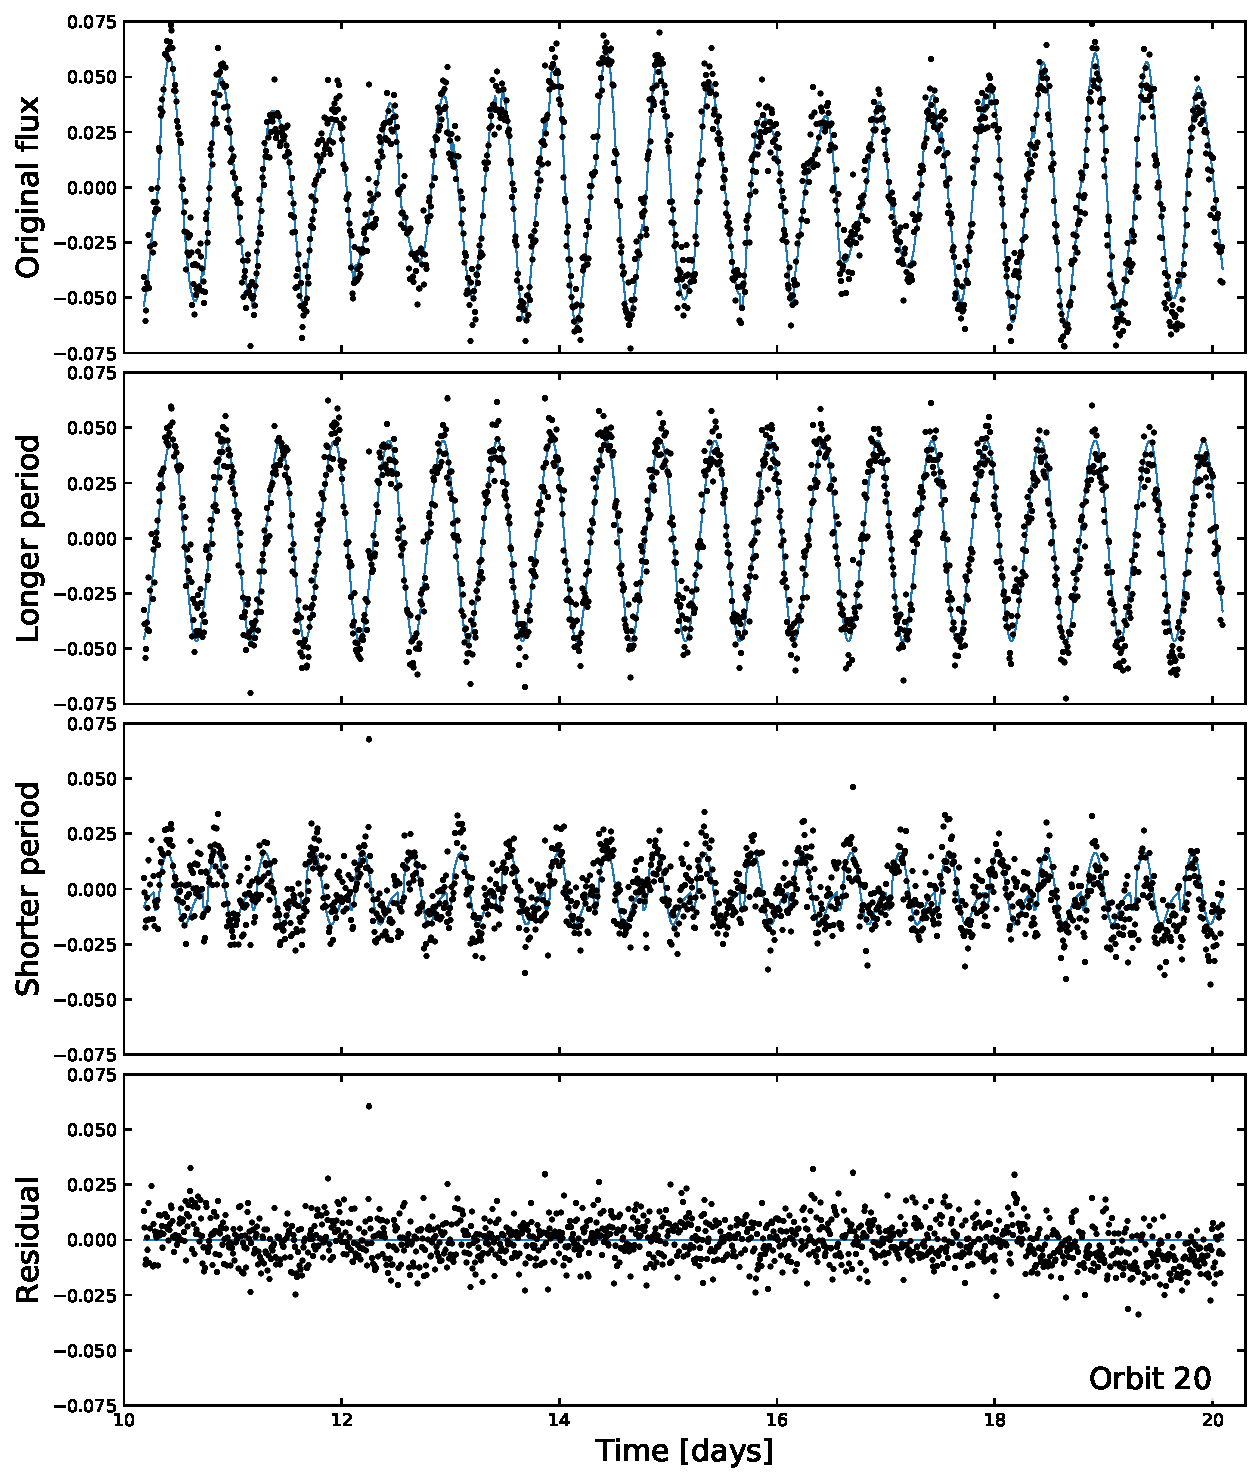
\includegraphics[width=0.95\textwidth]{f2.pdf}
	\end{center}
	\vspace{-0.7cm}
	\caption{ {\bf Phase-folded long and short-period signals.}
	{\it Top}: Long-period signal, as in Figure~\ref{fig:splitsignal}.
	{\it Bottom}: Short-period signal. The reference phase is set to the ``planetary'' dip.
	Gray points are the 10 minute cadence \texttt{PDCSAP} flux.
	Black points are binned to 100 points per period.
	\label{fig:phasefold}
	}
\end{figure*}


\begin{figure}[t]
	\begin{center}
		\leavevmode
		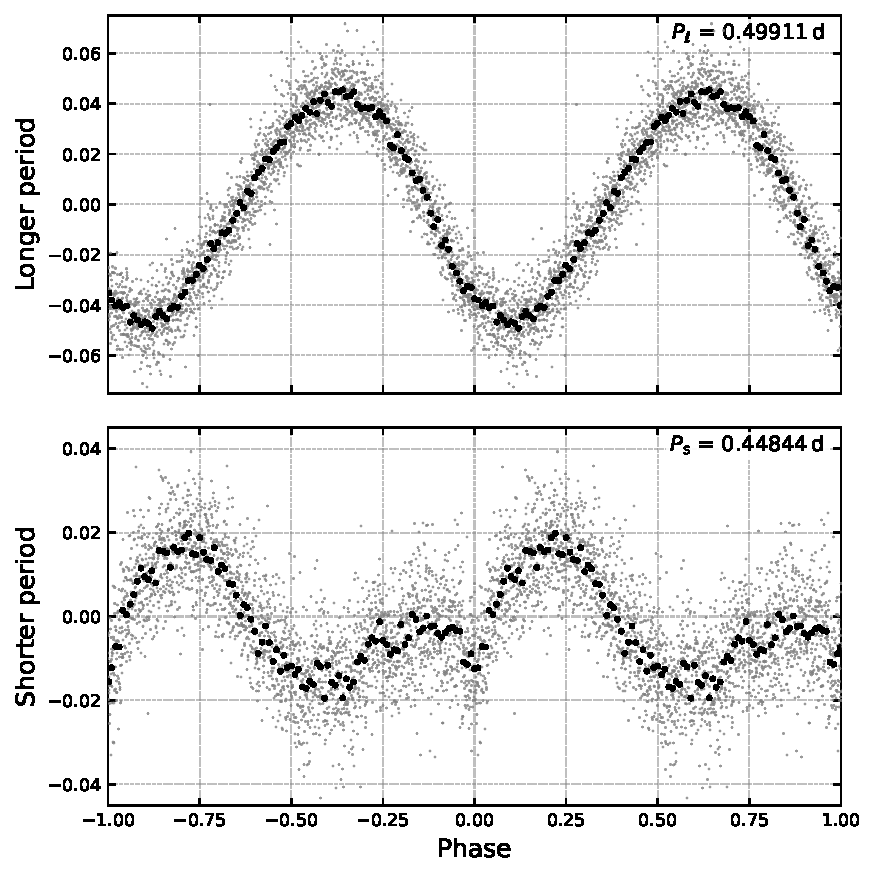
\includegraphics[width=0.48\textwidth]{f3.pdf}
	\end{center}
	\vspace{-0.7cm}
	\caption{ {\bf Scene used for blend analysis.}
		{\it Top:} Mean TESS image of PTFO 8-8695 over Sector~6, with a log-stretch.
		The position of PTFO 8-8695 is shown with a yellow star.
		Neighbors with $T<17$ are shown with orange crosses.
		The apertures used to measure the background and target star flux
		are shown with \texttt{X} and \texttt{/} hatches, respectively.
		{\it Bottom:} Digitized Sky Survey $R$-band image of the same field, with a linear stretch. The circles show
		apertures of radii 1, 1.5, and 2.25 pixels used in part of our blend
		analysis.
		The pixel level TESS data show that ``Star A''  does not contribute variability at either of the two observed periods (see Section~\ref{subsec:blend}).
		\label{fig:scene}
	}
\end{figure}

\begin{figure*}[t]
	\begin{center}
		\leavevmode
		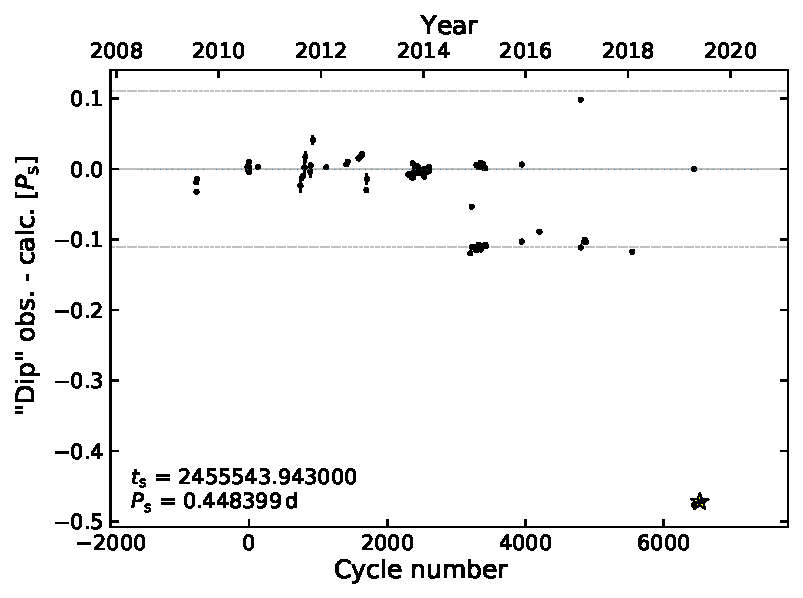
\includegraphics[width=0.9\textwidth]{f4.pdf}
	\end{center}
	\vspace{-0.7cm}
	\caption{
    {\bf Timing residuals for PTFO 8-8695b from a decade of monitoring.}
		Black points are times of ``dips'', minus the indicated linear ephemeris.
    The $y$-axis is given in units of phase for the
    short-period signal.
    The star shows the binned TESS ephemeris.
		``Dips'' have been observed by
		\citet{van_eyken_ptf_2012}, \citet{ciardi_follow-up_2015},
		\citet{yu_tests_2015}, \citet{raetz_yeti_2016},
		\citet{onitsuka_multi-color_2017}, and \citet{tanimoto_evidence_2020}.
    Certain dips ({\it e.g.}, the one at phase 0 in mid-2019) are
    consistent with noise, and were likely reported because
    something was {\it expected}, rather than convincingly {\it
    observed}.
    Horizontal dashed lines are drawn at $\pm (P_{\rm \ell} - P_{\rm s})/P_{\rm s}$,
    highlighting what could be either a numerical coincidence or an observational
    bias.
    The orbital phase observed by TESS is consistent with that of \citet{tanimoto_evidence_2020}, and quite different from the original phase.
		\label{fig:o_minus_c}
	}
\end{figure*}

\begin{figure*}[t]
	\begin{center}
		\leavevmode
		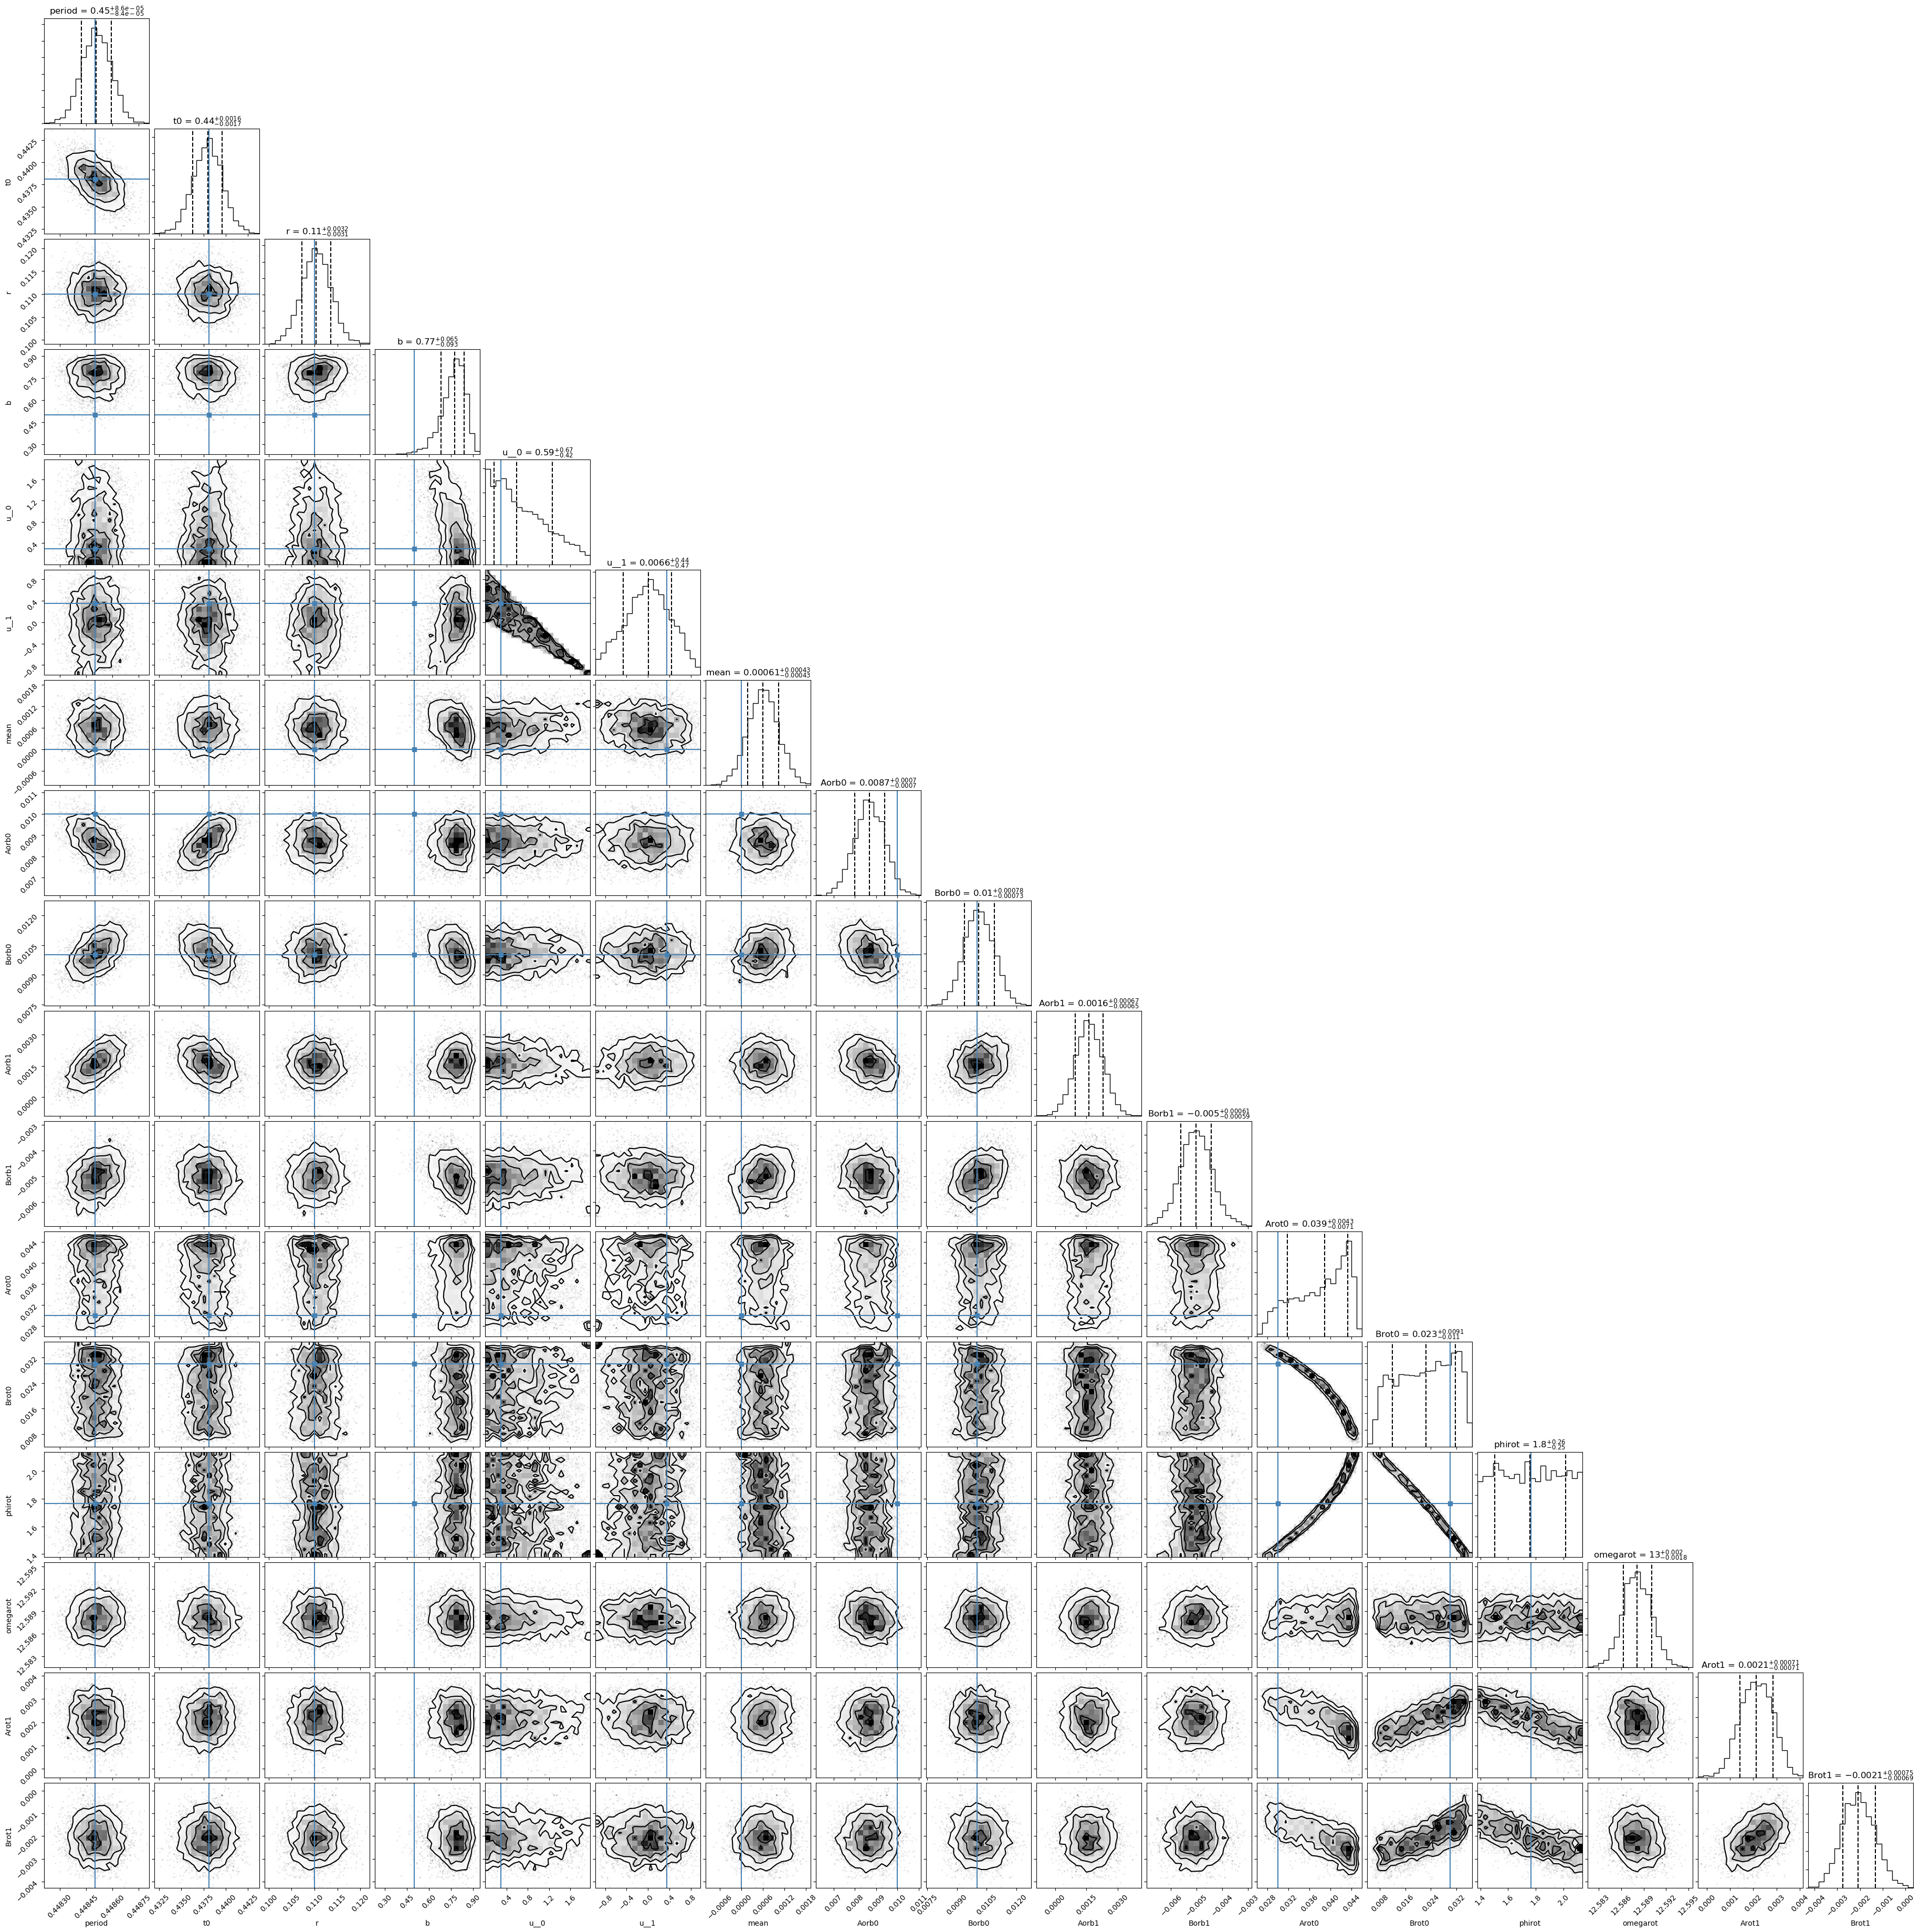
\includegraphics[width=0.9\textwidth]{f5_comp.png}
	\end{center}
	\vspace{-0.7cm}
	\caption{ {\bf foo.}
    bar
		\label{fig:corner}
	}
\end{figure*}


\subsection{Model Fitting}

We opted to model the lightcurve as a linear combination of Fourier
harmonics at the short and long periods, plus a transit at the short
period.  Symbolically,
\begin{equation}
  f = f_{\rm s} + f_{\rm \ell}
  = f_{\rm transit,s} + f_{\rm Fourier,s} + f_{\rm Fourier,\ell},
\end{equation}
where $f_{\rm s}$ is the relative flux at the short period, and
$f_{\rm \ell}$ is the flux at the long period.  Writing out the
Fourier terms,
\begin{align}
  f = &f_{\rm transit,s} + \sum_{n=1}^{n=N} A_n \sin(n\omega_{\rm s}t)
  + \sum_{n=1}^{n=N} B_n \cos(n\omega_{\rm s}t)\\
  &+ \sum_{m=1}^{m=M} A_m \sin(m[\omega_{\rm \ell}t+\phi_{\rm \ell}])
  + \sum_{m=1}^{m=M} B_m \cos(m[\omega_{\rm \ell}t+\phi_{\rm \ell}]), \nonumber
\end{align}
for $N$ and $M$ the total number of harmonics at the short and long
period, respective, $A_i$ and $B_i$ for each harmonic term, and
$\omega_i = 2\pi / P_i$ the angular frequency for $i$ the short or
long period index.  We fixed the ``phase-offset'' for the short period
signal to be zero, and let the reference time for the long period
signal float by introducing $\phi_{\rm \ell}$.  Since we did not a
priori know how many harmonics would be appropriate, we considered a
number of different choices for $N$ and $M$, and used the Bayesian
information criterion to choose the appropriate model.

As an example, one possible model could be a transit, plus $N=2$
harmonics of sines and cosines at the short period, plus $M=1$
harmonics at the long period.  In this case, the free parameters would
be as follows.  For the transit, we would fit for the impact
parameter, the planet-to-star radius ratio, two quadratic limb
darkening parameters, the planet orbital period (equal to the short
period), the reference time for the transit, and the mean flux.  There
would be 4 additional Fourier amplitudes at the short period, plus 2
Fourier amplitudes at the long period, and well as the long period
itself and its phase.  For this case, we therefore fitted 14 free
parameters.

We implemented the models using \texttt{PyMC3}, which is built on \texttt{theano} \citep{salvatier_2016_PyMC3,exoplanet:theano}.
For the Fourier terms, we used the default math operators.
For the exoplanet transit, we used the model and derivatives implemented in
\texttt{exoplanet} \citep{exoplanet:exoplanet}.

Our priors were as follows.
%FIXME

We initialized to the maximum a posteriori (MAP) solution.
We then sampled using \texttt{PyMC3}'s gradient-based No-U-Turns Sampler, 
and used R-hat as our convergence diagnostic.


% 
% I gave it a pass on the PTFO data, binning from 2->10 minute sampling
% to speed up the execution time. Results from two models are below.
% Case 1 is N=2,M=1. Case 2 is N=2,M=2. Both fits are fine, and I get
% decent convergence with a few minutes each. The rotation parameters
% (phase + amplitudes) are quite correlated, so I set a reasonably
% strong prior on the rotation phase.
% 
% The main result that both models agree on: the extra power at the
% orbital frequency seems to not be ellipsoidal. Both of these models
% prefer to put the power at 1x the orbital frequency, not 2x the
% orbital frequency! This gives both Aorb0 and Borb0 non-zero, while
% Aorb1 and Borb1 seem to be more consistent with zero.



% Using the cleaned PDC lightcurve, we applied the Box Least Squares
% algorithm \citep{kovacs_box-fitting_2002} to estimate the orbital
% period, transit duration, and a reference epoch using the TESS data
% alone.  Based on the results, we isolated the data within 4 transit
% durations of each transit midpoint.  To find the transit parameters
% that best fit the data, we first fitted a line to the out-of-transit
% flux measurements surrounding each transit, and divided it out.  We
% then created a phase-folded lightcurve \added{from all 18 transits}
% and fitted a standard transit model using the analytic formulae given
% by \citet{mandel_analytic_2002} and implemented by
% \replaced{\citet{kreidberg_batman_2015}}{\citet[][\texttt{BATMAN}]{kreidberg_batman_2015}}
% We assumed the orbit to be circular, consistent with the limits from
% radial velocities and occultation timing
% \citep{beerer_secondary_2011,knutson_friends_2014,bonomo_gaps_2017}.
% The free parameters were the reference epoch, the planet to star
% radius ratio $R_{\rm p}/R_\star$, the orbital distance to stellar
% radius ratio $a/R_\star$, the inclination $i$, two quadratic
% limb-darkening coefficients $(u_{\rm linear}, u_{\rm quad})$, and the
% orbital period $P$.
% 
% We sampled the posterior probability distribution for all the
% parameters using the algorithm proposed by
% \citet{goodman_ensemble_2010} and implemented by
% \replaced{\citet{foreman-mackey_emcee_2013}}{\citet[][\texttt{emcee}]{foreman-mackey_emcee_2013}}.
% Table~1 gives the results, which are in reasonable agreement with the
% parameters reported by {\it e.g.},
% \citet{southworth_high-precision_2009} and
% \citet{huitson_gemini_2017}.  Figure~\ref{fig:phasefold} shows the
% phase-folded lightcurve.
% 
% To measure the transit times, we returned to the `cleaned' PDC time
% series and fitted the data within four transit durations of each
% transit separately. We used four free parameters: the time of
% mid-transit $t_{\rm tra}$, the planet-to-star radius ratio, and the
% slope and intercept of a linear trend to account for any slow
% variations unrelated to the transit.  We fixed the remaining
% parameters at the values that had been determined from the
% phase-folded TESS lightcurve.  The uncertainty in each
% \added{photometric} data point was set equal to the root-mean-square
% (rms) level of the out-of-transit data.
% 
% To verify that the measured uncertainties are estimated accurately, we
% computed the \deleted{reduced }$\chi^2$\added{ value} for a linear
% ephemeris fit to the measured TESS mid-transit times.  We found that
% $\chi^2 = 9.2$, with $n=16$ degrees of freedom.  The variance of the
% $\chi^2$ distribution is $2n$, so we would expect $\chi^2 = 16 \pm
% 5.7$.  Visually inspecting the residuals showed that the error
% variance had been overestimated, so we multiplied the measured TESS
% errors by a factor $f=0.76$, forcing a reduced $\chi^2$ of unity.
% This lowered the mean uncertainty of the transit midtimes from $29.8$
% to $22.6$ seconds.  We verified that omitting this step did not
% appreciably alter any of our conclusions.
% 
% Figure~\ref{fig:lightcurves} shows the lightcurve of each individual
% transit, the best-fit models, and the residuals.  Table~2 reports the
% mid-transit times and their uncertainties.  After binning the
% residuals to 1-hour windows, the lightcurves have an rms scatter of
% 586\,{\rm ppm}.  The pre-launch TESS noise
% model\footnote{\url{github.com/lgbouma/tnm}, commit \texttt{be06f09}}
% (\citealt{winn_photonflux_2013}, \citealt{Sullivan_2015} Section 6.4)
% would have predicted an error budget consisting of the following terms
% added in quadrature: 410\,{\rm ppm} from photon-counting noise,
% 202\,{\rm ppm} from detector read noise, and 673\,{\rm ppm} from the
% zodiacal background light.  The level of background light appears to
% have been overestimated in the model.



% I fitted some models of the form "transit + N harmonics of sines and
% cosines at the orbital frequency + M harmonics of sines and cosines at
% the rotation frequency". For example, if N=2 and M=1, then I fit for
% [logBrot0, logArot0, phirot, omegarot, logBorb1, logAorb1, logBorb0,
% logAorb0, b, r, u, logP, t0, meanflux]. A_N is the amplitude of the
% Nth harmonic sine function A_N * sin(N(ωt+φ)), B_N of the cosine. I
% went with quadratic limb darkening.
% 
% On fake data, I got the right parameters provided I didn't turn up the
% noise too high.
% 
% I gave it a pass on the PTFO data, binning from 2->10 minute sampling
% to speed up the execution time. Results from two models are below.
% Case 1 is N=2,M=1. Case 2 is N=2,M=2. Both fits are fine, and I get
% decent convergence with a few minutes each. The rotation parameters
% (phase + amplitudes) are quite correlated, so I set a reasonably
% strong prior on the rotation phase.
% 
% The main result that both models agree on: the extra power at the
% orbital frequency seems to not be ellipsoidal. Both of these models
% prefer to put the power at 1x the orbital frequency, not 2x the
% orbital frequency! This gives both Aorb0 and Borb0 non-zero, while
% Aorb1 and Borb1 seem to be more consistent with zero.

The periodogram of the final residual (Figure~\ref{fig:splitsignal}
bottom row) shows a weakly significant, poorly resolved peak at
$\approx$8 days, consistent with the visual impression in the time
domain that there could be a weak long-period signal present.


\subsection{Blend considerations}
\label{subsec:blend}

The TESS pixels are $\approx21$'' per side, and so we need to consider
whether light from neighboring stars could affect the photometry.  The
scene is shown in Figure~\ref{fig:scene}.  
The pixels used to
measure the background level are indicated with an `\texttt{X}' hatch,
and the pixels used for the final lightcurve are shown with the
`\texttt{/}' hatch.

The target star, PTFO
8-8605 (TIC 264461976), has a $T$-band magnitude of 14.0, and its position is shown with a
star.  
The other (unlabeled) star inside the target aperture, TIC 264461979, has $T=16.8$ and so cannot
contribute a signal with relative amplitude 10\%.
The only neighbor that is sufficiently close and bright that
its light might contaminate the target star is TIC 264461980, with
$T=14.8$, which we denote ``Star A''.  Star A is 23.6'' NW of our
target, and based on the magnitude difference could contribute up to
48\% the flux of our target star, PTFO 8-8695.  

Because PTFO 8-8695 has previously been identified to have periodicity
consistent with our measurement of $P_{\rm s}$, our main concern
regarding blending is the degree to which we can be certain that the
long-period signal at $P_{\rm \ell}$ also originates from PTFO 8-8695.
We took two approaches towards determining the source of the long-period signal.

First, we examined the CDIPS full frame image lightcurves of the
target, which are available on MAST \citep{bouma_cluster_2019}.
The maximal peak-to-peak beat amplitude is consistently $\approx$10\%
across apertures of radii 1, 1.5, and 2.25 pixels.
If Star A were the source of the long-period variability, we would expect the
peak variability amplitude to be smallest in the 1 pixel aperture, based on the
separation of the sources (Figure~\ref{fig:scene}, bottom).
From this test alone, it seems unlikely that Star A is the source of
the long-period signal.

Second, we examined the lightcurve of each pixel in the scene
individually.  We opted to use the
interactive tools implemented in
\texttt{lightkurve} \citep{lightkurve_2018}.  If Star A were the
source of the long-period variability, we would expect the pixels
nearest to Star A to show a sinusoidal signal with
amplitude exceeding $10\%$.  We find no evidence for
this being the case.  The pixel directly below Star A does not
clearly show the sinusoidal variability, and the peak-to-peak 
variability in that pixel is $\lesssim 8\%$.  In contrast, the
south-easternmost pixel within PTFO 8-8695's aperture (the pixel 
furthest from Star A that was used in the optimal aperture) shows the $P_{\rm \ell}$ sinusoidal
variability signal at $\approx 10\%$ amplitude.

As there is no evidence in favor of a blend scenario, we
conclude that both the $P_{\rm s}$ and $P_{\rm \ell}$ signals originate from PTFO 8-8695.

\section{Interpretation}
\label{sec:discussion}

The TESS dip does not phase up where it is supposed to...
\label{fig:o_minus_c}

\section{Conclusions}
\label{sec:conclusions}



%%%%%%%%%%%%%%%%%%%%%%%%%%%%%%%%%%%%%%%%%%%%%%%%%%%%%%%%%%%%%%%%%%%%%%%%%%%%%%%

% \acknowledgements
% %
% This paper includes data collected by the TESS mission, which are
% publicly available from the Mikulski Archive for Space Telescopes
% (MAST).
% %
% Funding for the TESS mission is provided by NASA's Science Mission
% directorate.
% %
% This work made use of NASA's Astrophysics Data System Bibliographic
% Services.
% %
% Based on observations obtained at the Gemini Observatory, which is
% operated by the Association of Universities for Research in Astronomy,
% Inc., under a cooperative agreement with the NSF on behalf of the
% Gemini partnership: the National Science Foundation (United States),
% National Research Council (Canada), CONICYT (Chile), Ministerio de
% Ciencia, Tecnolog\'{i}a e Innovaci\'{o}n Productiva (Argentina),
% Minist\'{e}rio da Ci\^{e}ncia, Tecnologia e Inova\c{c}\~{a}o (Brazil),
% and Korea Astronomy and Space Science Institute (Republic of Korea).
% %
% Observations in the paper made use of the High-Resolution Imaging
% instrument Zorro at Gemini-South. Zorro was funded by the NASA
% Exoplanet Exploration Program and built at the NASA Ames Research
% Center by Steve B. Howell, Nic Scott, Elliott P. Horch, and Emmett
% Quigley.
% %
% This research has made use of the VizieR catalogue access tool, CDS,
% Strasbourg, France. The original description of the VizieR service was
% published in A\&AS 143, 23.
% %
% This work has made use of data from the European Space Agency (ESA)
% mission {\it Gaia} (\url{https://www.cosmos.esa.int/gaia}), processed
% by the {\it Gaia} Data Processing and Analysis Consortium (DPAC,
% \url{https://www.cosmos.esa.int/web/gaia/dpac/consortium}). Funding
% for the DPAC has been provided by national institutions, in particular
% the institutions participating in the {\it Gaia} Multilateral
% Agreement.
%
% (Some of) The data presented herein were obtained at the W. M. Keck
% Observatory, which is operated as a scientific partnership among the
% California Institute of Technology, the University of California and
% the National Aeronautics and Space Administration. The Observatory was
% made possible by the generous financial support of the W. M. Keck
% Foundation.
% The authors wish to recognize and acknowledge the very significant
% cultural role and reverence that the summit of Maunakea has always had
% within the indigenous Hawaiian community.  We are most fortunate to
% have the opportunity to conduct observations from this mountain.
%
% \newline
%

\software{
  \texttt{astrobase} \citep{bhatti_astrobase_2018},
  % \texttt{astroplan} \citep{astroplan2018},
  \texttt{astropy} \citep{astropy_2018},
  \texttt{astroquery} \citep{astroquery_2018},
  % \texttt{BATMAN} \citep{kreidberg_batman_2015},
  \texttt{corner} \citep{corner_2016},
  %\texttt{emcee} \citep{foreman-mackey_emcee_2013},
  \texttt{exoplanet} \citep{exoplanet:agol19}
  \texttt{exoplanet} \citep{exoplanet:exoplanet}, and its
  dependencies \citep{exoplanet:agol19, exoplanet:kipping13, exoplanet:luger18,
  	exoplanet:theano}.
  \texttt{IPython} \citep{perez_2007},
	\texttt{lightkurve} \citep{lightkurve_2018},
  \texttt{matplotlib} \citep{hunter_matplotlib_2007}, 
  \texttt{MESA} \citep{paxton_modules_2011,paxton_modules_2013,paxton_modules_2015}
  \texttt{numpy} \citep{walt_numpy_2011}, 
  \texttt{pandas} \citep{mckinney-proc-scipy-2010},
  \texttt{PyMC3} \citep{salvatier_2016_PyMC3},
  \texttt{radvel} \citep{fulton_radvel_2018},
  % \texttt{scikit-learn} \citep{scikit-learn},
  \texttt{scipy} \citep{jones_scipy_2001}.
}


% \facilities{
% 	{\it Astrometry}:
% 	Gaia \citep{gaia_collaboration_gaia_2016,gaia_collaboration_gaia_2018}.
% 	{\it Imaging}:
% 	Gemini:South~(Zorro; \citealt{scott_nessi_2018}.
% 	{\it Spectroscopy}:
% 	Keck:I~(HIRES; \citealt{vogt_hires_1994}),
% 	Euler1.2m~(CORALIE),
% 	ESO:3.6m~(HARPS; \citealt{mayor_setting_2003}).
% 	{\it Photometry}:
% 	CTIO:1.0m (Y4KCam),
% 	Danish 1.54m Telescope,
% 	El Sauce:0.356m,
% 	Elizabeth 1.0m at SAAO,
% 	Euler1.2m (EulerCam),
% 	Magellan:Baade (MagIC),
% 	Max Planck:2.2m	(GROND; \citealt{greiner_grond7-channel_2008})
% 	NTT,
% 	SOAR (SOI),
% 	TESS \citep{ricker_transiting_2015},
% 	TRAPPIST \citep{jehin_trappist_2011},
% 	VLT:Antu (FORS2).
% }

%
% The following are entries from Table 1 that are not otherwise cited
% in the text
%
% \nocite{wilson_wasp-4b_2008}
% \nocite{gillon_improved_2009}
% \nocite{winn_transit_2009}
% \nocite{hoyer_tramos_2013}
% \nocite{dragomir_terms_2011}
% \nocite{sanchis-ojeda_starspots_2011}
% \nocite{nikolov_wasp-4b_2012}
% \nocite{ranjan_atmospheric_2014}
% \nocite{huitson_gemini_2017}

% \input{WASP-4b_transit_time_table.tex}
% \input{WASP-4b_rv_table.tex}
% \input{model_fit_table.tex}
% \input{rv_model_posterior_table.tex}
% \input{pdot_table.tex}

%\clearpage
\bibliographystyle{yahapj}                            
\bibliography{bibliography} 


\listofchanges

\end{document}
